\chapter{Introduction}
Quality of Service (QoS) is the resource reservation control mechanism in place to guarantee a certain level of performance and availability of a service. It provides a level of assurance that the resource requirements of an application are strictly supported \cite{QOS}. It is possible that the resource requirement of a user may not be supported by the cloud provider. In such 
scenarios, the cloud provider has to provide a means of executing the user's load. The provider has to decide the appropriate strategy such that the user's needs are met. One of the most interesting aspects in Cloud Computing is the feeling of availability of `infinite' computing resources that the cloud provider tries to distribute to the user in an elastic way \cite{RAD}. The user does not fully realize the internal allocations while demanding for more resources.
\begin{center}
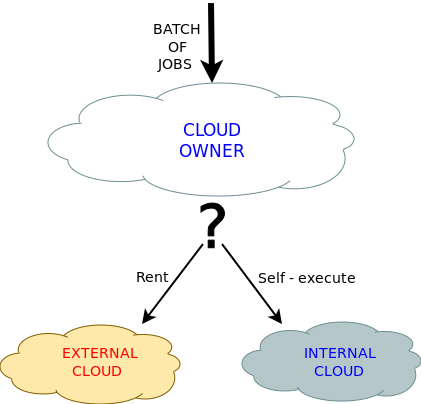
\includegraphics[width=0.75\textwidth]{Diagram1}\\[0.3cm]
\end{center}
For this infinite demand of the user to be met, the cloud provider has to find ways to do it without incurring any loss. One of the approaches to do it is to calculate the number of times the provider does not have the capacity to execute the load and based on that draw up an agreement with another provider to execute the load. This calculation can be predicted from past data through forecasting and by game theory (to include the current data also). The method of standard deviation can help in deciding the strategy of the cloud provider.
\section{Problem Statement}
Identification of a Rent or Self-execute strategy in Clouds for an incoming batch of jobs. The strategy adopted defines when a Cloud owner decides whether a batch can be executed using an internal Cloud or has to pay rent to execute it in an external Cloud provider.
\begin{itemize}
\item Use of forecasting methods to predict the strategy. 
\item Applying a game theoretic approach to decide the strategy.
\item Use the above two approaches to decide on one final strategy.
\end{itemize}

